\chapter{Discussion}
	\label{discussion}
	The process described in this Report offers a way of creating boundary representations of indoor scans without the need for user interference or preprocessing of the cloud. Section \ref{Comparison} shows that the resulting boundary representation of the room does not differ from the real room by much at all even though the scan is very noisy and even has one wall made up mostly of windows and blinds. 
	
	\begin{figure}[H]
	\centering
	\includegraphics[width=0.9\linewidth]{"Includes/images/Results/Messy Wall"}
	\caption{Objects and blinds obscuring the left hand wall}
	\label{fig:MessyWall}
	\end{figure}
	
	
	\section{Comparison of model to Real Measurements}
		\label{Comparison}
		In determining if the resulting Boundaries are correct, and a good representation of the room that has been scanned, measurements were taken of the room with a distometer and corresponding measurements were taken on the model. the results of this comparison can be seen in table \ref{MeasurmensTable}. 
		
		\begin{table}[H]
			\centering
			\begin{tabular}{|c|c|c|c|}
				\hline m & Distometer & Model & Difference \\ 
				\hline 1 & 7.205 & 7.208 & 0.003 \\ 
				\hline 2 & 5.426 & 5.420 & 0.006 \\ 
				\hline 3 & 7.203 & 7.206 & 0.003 \\ 
				\hline 4 & 5.422 & 5.427 & 0.005 \\ 
				\hline H 1 & 2.492 & 2.495 & 0.003 \\ 
				\hline H 2 & 2.495 & 2.497 & 0.002 \\ %TODO get actual disto for heights
				\hline
			\end{tabular}
			\caption{Measurements with a distometer versus measurements taken on the model}
			\label{MeasurmensTable}
		\end{table}
		
		
		\begin{figure}[H]
			\centering
			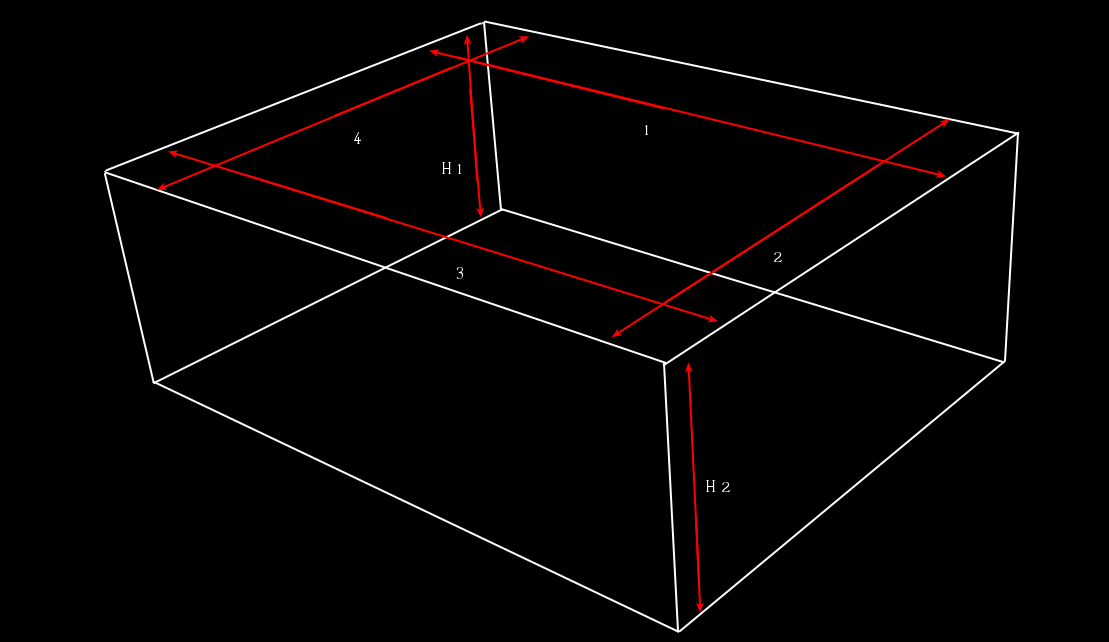
\includegraphics[width=0.7\linewidth]{Includes/images/Results/Selection_013}
			\caption{Locations of the measurements in Table \ref{MeasurmensTable}}
			\label{fig:SourceOfMEasure}
		\end{figure}
		
		\noindent It is important to note that the Oriented bounding box of the room has the dimensions 5.795m, 7.455m, 2.900m. The OBB is therefore 37cm bigger along the width of the room, 25cm in the length and 40cm bigger vertically. This is important because it may look like a bounding box has been created but that is not the case.
		
	\section{Plane Fitting accuracy}
		Having planes fitted to each planar segment is a key part of the process, the accuracy of these fitted planes is vital to having accuracy in the final output. Figure \ref{fig:Planefitingaccuracy} shows how a segment varies from the fitted plane on the right hand wall. The error ranges from perfect fit, shown in red, to an error of 10mm in the blue section at the top left.
		
		\begin{figure}[H]
		\centering
		\includegraphics[width=1\linewidth]{"Includes/images/Results/Plane fiting accuracy"}
		\caption{Blue to Red scale of point variance from fitted plane on right hand wall segment }
		\label{fig:Planefitingaccuracy}
		\end{figure}
	
	\section{Limitations of this process}
		As it stands the main limitations on this process are the complexity of the room that is scanned. Rooms that are reasonably rectangular can be processed successfully. But as soon as small sections start to kink out or there are walls that start to run at different angles the Extrusion method explained in section \ref{Extrusion} fails. This, as well as networks of rooms will be discussed further in the Conclusions and Future work section.
		
	\section{File Size}
		A major benefit for this system is that a large point cloud can be greatly reduced in size without loosing any of the main information about the room. 
		
		
		
		START = 25mb - 1,061,000pts
		\\
		end  = 1.3k - 24pts
	
	
\chapter{Conclusions and Future work}

conclusions..

\section{Future Work}
	The process described in this report is still in its infancy, and has a few limitations. The ideas in this Report can continue to be extended into more complex rooms and then into multiple rooms, essentially a network of interconnected rooms. \cite{mura_automatic_2014} have shown a very successful method for dealing with multiple rooms.
	
	Another possible road to go down is the start creating more detail in the 3D models created. For instance showing the location of windows and doors in the in the CAD models.
	
